\begin{figure}[!t]
	  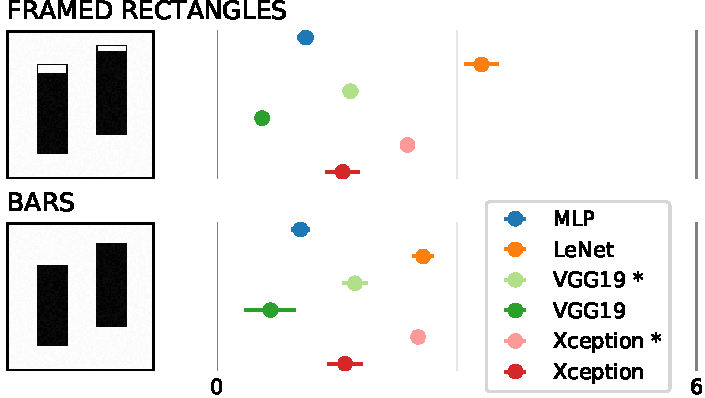
\includegraphics[width=\linewidth]{figure12_mlae_better_all.pdf}
  \caption{\textbf{Computational results of the bars-and-framed-rectangles experiment.} \textit{Left:} Visual encodings of two bars for a task of length judgement (bottom) following Cleveland and McGill's proposed experiment. Perceiving which bar is longer is much easier for humans when a frame is added (top). For networks (trained from scratch, or * indicates ImageNet weights), there seems no significant difference between the encodings as reported by MLAE and 95\% confidence intervals.}
	\label{fig:figure12_mlae}
\end{figure}


\section{Experiment: Bars and Framed Rectangles}

Visual cues can help converting graphical elements back to their real world variables. Cleveland and McGill introduced the bars-and-framed-rectangles experiment which compares the perceptual judgement tasks  of length and position along non-aligned scales~\cite{cleveland_mcgill}. Figure~\ref{fig:figure12_mlae} shows both variations on the left. It is not easy to judge which bar is larger in the bottom picture which involves a length judgement. However, when adding a little frame as a reference, this length judgement is transferred to a position judgement along non-aligned scales. Based on this little frame, it is easy to see that the right bar is slightly larger than the left since the whitespace in the top of the frame is smaller than the one on the left. 

As Cleveland and McGill explain in their theories, judging the whitespace is actually also a length judgement rather than a position~\cite{cleveland_mcgill}. They now relate this task to Weber's Law which states that the perceivable difference within a distribution is proportional to the initial size of the distribution~\cite{householder1940weber}. Here, it means that humans can easily measure the difference in the white scale since its initial size is small while estimating the small change in lengths of the black bars is not easily perceivable. The Just Noticable Difference (JND) is higher when the initial stimuli is smaller in size (here the white bars).

We mimmick the bars-and-framed rectangles experiment as a two value regression task. We create rasterized visualizations of size $100\times100$ as shown in Figure~\ref{fig:figure12_mlae} and let our networks estimate the sizes of the stimuli.

\subsection{Hypotheses}

We proposed two hypotheses entering the elementary perceptual task experiment:

\begin{itemize}
	\item \textbf{H4.1} \textbf{Classifiers can leverage additional visual cues.} The original bar and framed rectangle experiment shows how visual cues aid humans in mapping graphical elements to quantitative variables. This should be the same for feed-forward neural networks since they are inspired by the visual system.
	\item \textbf{H4.2} \textbf{Weber's law can be transferred to computational perception.} Cleveland and McGill confirmed Weber's law based on the bar and framed rectangle experiment. For humans, the ability to perceive change within a distribution is proportional to the size of the initial distribution.
\end{itemize}

%\begin{figure}[t]
%	  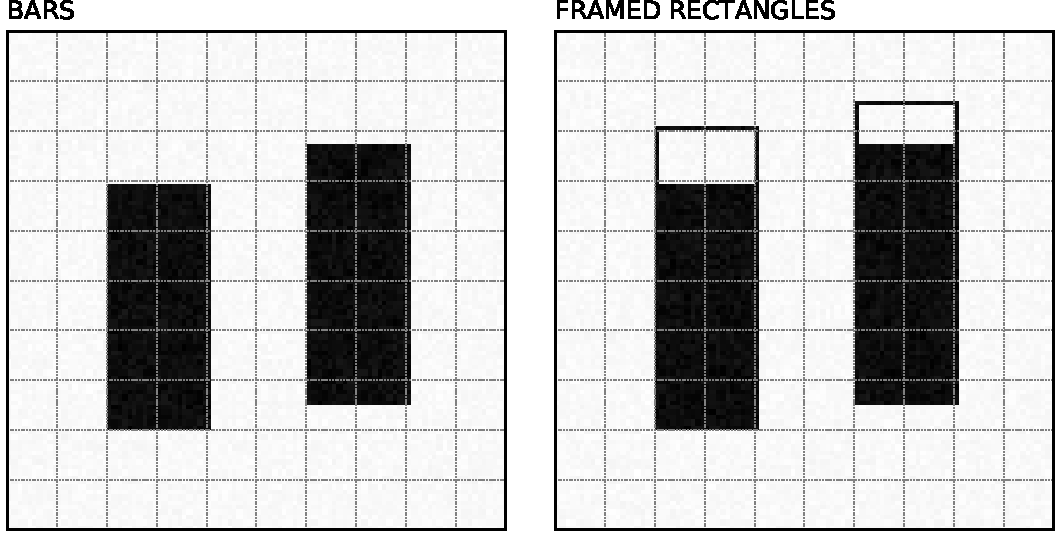
\includegraphics[width=\linewidth]{figure12_overview}
%  \caption{\textbf{Bars and Framed Rectangles Experiment.} Cleveland and McGill introduce the bars and framed rectangles experiment which measures the perceptual task of judging position along non-aligned scales. For humans, it is easier to decide which of two bars represent a larger height if a scale is introduced by adding framed rectangles (right). In this case, the right bar is heigher as visible with less free space when adding the frame. We evaluate whether such a visual aid also helps machines to perceive visually encoded quantities.}
%	\label{fig:bars_and_framed_rectangles_experiment}
%\end{figure}
%\begin{table}[h]
%\centering
%\caption{\textbf{Bars and Framed Rectangles Experiment.} Cleveland and McGill introduce the bars and framed rectangles experiment which measures the perceptual task of judging position along non-aligned scales. For humans, it is easier to decide which of two bars represent a larger height if a scale is introduced by adding framed rectangles. In this case, the right bar is heigher as visible with less free space when adding the frame. We evaluate whether such a visual aid also helps machines to perceive visually encoded quantities.}
%\resizebox{\linewidth}{!}{
%\begin{tabular}{lllr}
%	\toprule
%	\multicolumn{2}{l}{~} & ~ & Permutations\\
%
%	\midrule
%	\raisebox{-.85\height}{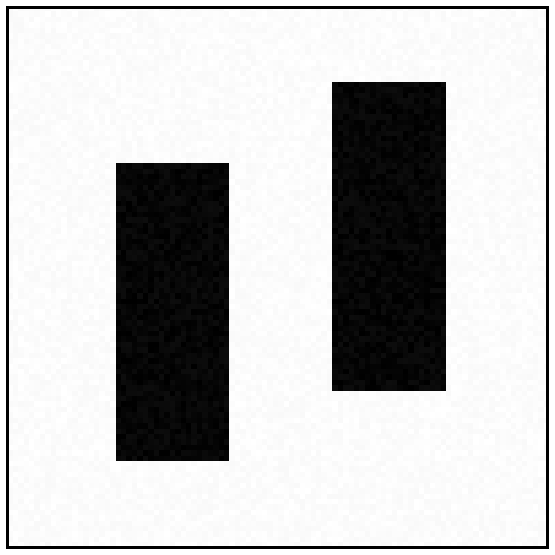
\includegraphics[width=.5in]{figure12_0.pdf}} & \makecell[tl]{\emph{Bars}\\~~~Perceptual Task: \emph{Length}\\~~~JND: $X\%$\\~ \\~~~~~~~~~~~~~~~~~~~~~~~~~~~~~~~~ \\} &~& \makecell[tr]{~\\ $57,600$}\\
%
%
%	\midrule
%	\raisebox{-.85\height}{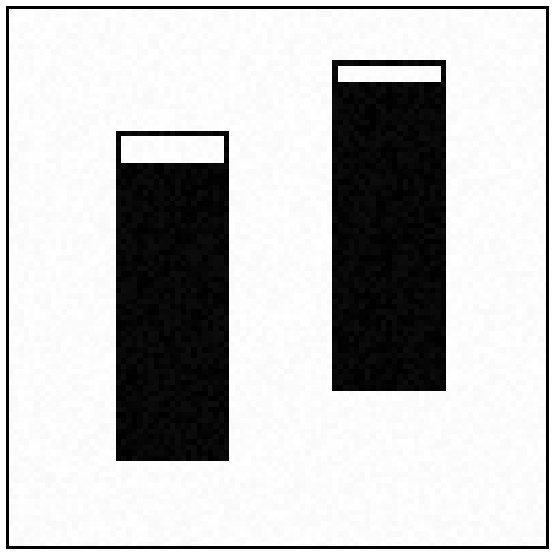
\includegraphics[width=.5in]{figure12_1.pdf}} & \makecell[tl]{\emph{Framed Rectangles}\\~~~Perceptual Task: \emph{Position}\\~~~JND: $X\%$\\~ \\~~~~~~~~~~~~~~~~~~~~~~~~~~~~~~ \\} &~& \makecell[tr]{~\\ $57,600$}\\
%
%
%	\bottomrule
%\end{tabular}
%}
%\label{tab:bars_and_framed_rectangles_parameters}
%\end{table}




%\begin{figure}[t]
%	  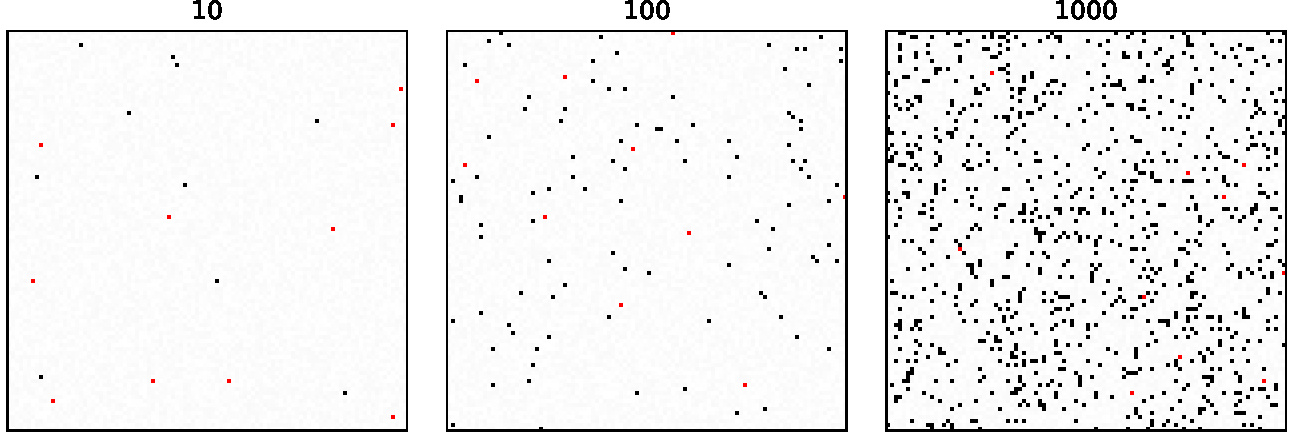
\includegraphics[width=\linewidth]{weber_overview}
%  \caption{\textbf{Weber-Fechner Law.} The Weber-Fechner law states that the perceivable differences within a distribution is proportional to the initial size of the distribution. The lower square contains 10 more dots than the upper one on both sides. However, the difference is easily perceivable on the left while the squares on the right almost look the same. We generate rasterized visualizations similar to this setup and evaluate our classifiers.}
%	\label{fig:webers_law}
%\end{figure}
%\begin{table}[h]
%\centering
%\caption{\textbf{Weber-Fechner Law.} The Weber-Fechner law states that the perceivable differences within a distribution is proportional to the initial size of the distribution. We create three different types of images initialized with 10, 100, and 1000 dots. We then mark randomly up to 10  dots in previously free pixels (here visualized in red). For humans, the difference is easily perceivable when the initial dot count is 10 but is hard when it is higher. We evaluate our classifiers on these rasterized visualizations.}
%\resizebox{\linewidth}{!}{
%\begin{tabular}{lllr}
%	\toprule
%	\multicolumn{2}{l}{~} & ~ & Permutations\\
%
%	\midrule
%	\raisebox{-.85\height}{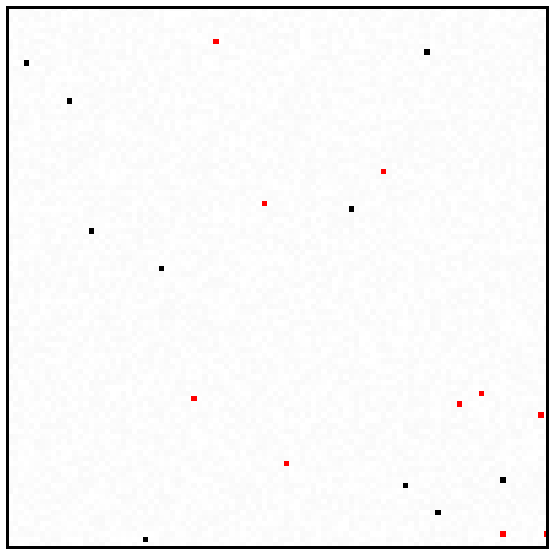
\includegraphics[width=.5in]{weber_0.pdf}} & \makecell[tl]{\emph{Base 10}\\~~~JND: $X\%$\\~ \\ ~~~~~~~~~~~~~~~~~~~~~~~~~~~~~~~~~~~~~~~~ \\} &~& \makecell[tr]{~\\ $10,000$}\\
%
%
%	\midrule
%	\raisebox{-.85\height}{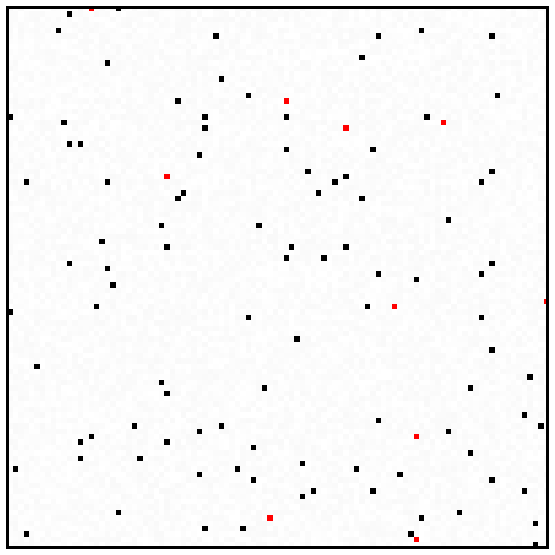
\includegraphics[width=.5in]{weber_1.pdf}} & \makecell[tl]{\emph{Base 100}\\~~~JND: $X\%$\\~ \\ ~~~~~~~~~~~~~~~~~~~~~~~~~~~~~~~~~~~~~~~~ \\} &~& \makecell[tr]{~\\ $10,000$}\\
%	
%	\midrule
%	\raisebox{-.85\height}{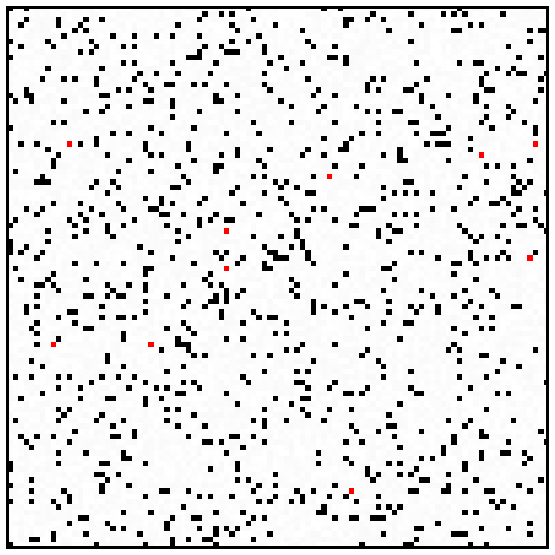
\includegraphics[width=.5in]{weber_2.pdf}} & \makecell[tl]{\emph{Base 1000}\\~~~JND: $X\%$\\~ \\ ~~~~~~~~~~~~~~~~~~~~~~~~~~~~~~~~~~~~~~~~ \\} &~& \makecell[tr]{~\\ $10,000$}\\
%
%	\bottomrule
%\end{tabular}
%}
%\label{tab:weber_law}
%\end{table}


\subsection{Point Cloud Experiment}

We conduct an additional experiment testing whether Weber's law applies to convolutional neural networks for graphical perception. For this, we generate three 2D point clouds as base stimuli -- each is created randomly by activating 10, 100, or 1000 pixels in a $100\times100$ raster image. We then additionally activate from 1 to 10 random pixels within the initial distribution but by carefully only selecting inactive pixels. We show examples for this in Figure~\ref{fig:weber_law} (left). This means that the number of additional points is harder to identify if they are added to the 1000 pixel set while the 10 pixel set allows to easily count. We then let our networks solve a regression task to estimate the number of added points.


\subsection{Results}



\begin{figure}[t]
	  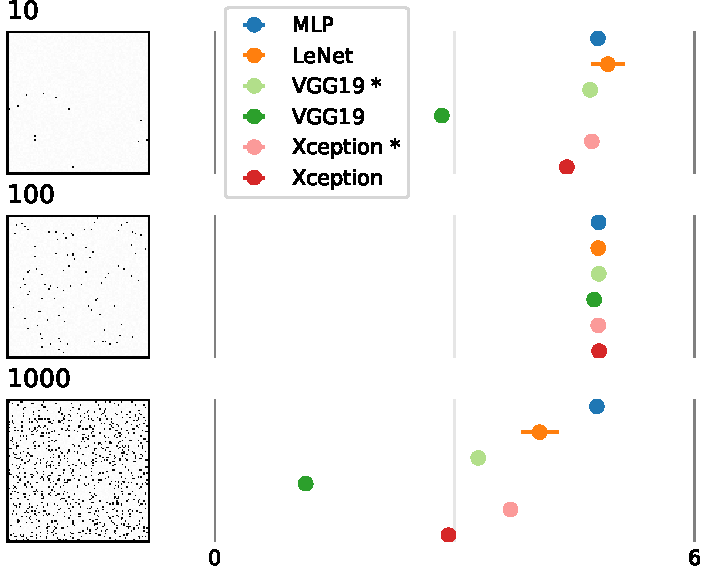
\includegraphics[width=\linewidth]{weber_mlae_noise_all.pdf}
  \caption{\textbf{Computational results of the point cloud experiment.} Log absolute error means and 95\% confidence intervals for the \emph{bars-and-framed-rectangles experiment} as described by Cleveland and McGill~\cite{cleveland_mcgill}. We test the performance of a Multi-layer Perceptron (MLP), the LeNet Convolutional Neural Network, as well as feature generation using the VGG19 and Xception networks trained on ImageNet.}
	\label{fig:weber_law}
\end{figure}
